\documentclass{article}
\usepackage{graphicx}
\usepackage{algorithm}
\usepackage[noend]{algorithmic}
\usepackage{subfigure}
\usepackage{amssymb, amsmath, graphicx, charter, latexsym}
\usepackage{layouts}
\usepackage[letterpaper]{geometry}
\usepackage{enumerate}
\usepackage{epstopdf}
\usepackage{ragged2e}
%\usepackage{times}
\usepackage{mathtools}
%\usepackage[scaled]{helvet}
\usepackage{mathptmx}
\usepackage{verbatim}
\usepackage{listings}
\usepackage{siunitx}
\usepackage{booktabs}
\usepackage{array}
\newcolumntype{P}[1]{>{\centering\arraybackslash}p{#1}}

\lstset{
basicstyle=\ttfamily,
}
\lstMakeShortInline|

\begin{document}

\title{\bfseries ECEN 689 -- Real-Time Wireless Networks: Project 3\\
Smart Scheduling with Point Coordination Function\\
 for WiFi Uplink Transmissions}
\date{Due on 4/6}
\author{%
Ping-Chun Hsieh\\
\texttt{lleyfede@tamu.edu}
\and
Tao Zhao\\
\texttt{alick@tamu.edu}
\and
Dongni Han\\
\texttt{handongni2015@tamu.edu}
}
\maketitle

\section*{Terminology}

In our report, we use AP or ``server'' to denote the WiFi access point, and ``client'' to denote the terminal device such as a mobile phone, a tablet, and so on. Throughout our simulation, we let node $0$ be the server, and the other nodes be the clients. The basic time unit for packet transmission is called \emph{slot}, which should be greater than a round-trip time (RTT). For real-time traffic, we group an integer number (denoted by $T$) of slots into an \emph{interval}, which is the relative deadline of the packets.

\section{Background}

We consider a wireless network of one AP and $N$ clients, where $N\ge1$. We consider uplink transmission with point coordination function (PCF). For uplink transmission, packets are generated by each client $n$ in each interval. Number of packets $X_n$ follows uniform distribution \{ $U_{min}$, $U_{max}$ \}. And we only consider real-time traffic. In PCF mode, AP polls at most one client per slot and it has full control over channel allocation. In the beginning of each interval, each client generates a random number of packets and waits for channel access that is fully controlled by the AP. Since the packets are generated and queued on the client's side, the AP needs to collect the queue information of the clients to make scheduling decisions.

With a baseline policy, in the phase 1,  the AP collects the queue information by polling each client one by one for the number of data packets it generates ($X_n$). After all clients are polled, the AP knows the number of packets at each client. In the phase 2, the AP uses Max-Weight scheduling to choose one of the clients in each time slot for actual data transmission. However, there are three issues about baseline policy. Firstly, no data transmissions is in phase 1. Secondly, channel utilization for data packets is very low. Thirdly, overhead is especially low when the number of clients $N$ is large or the channel is very poor because the AP spends much time on polling number in phase 1. 

\section{Smart Policy}

We use three different features to improve performance under symmetric and asymmetric channel. All combinations of three features are possible. And we use binary to represent those combination.
\begin{table}[htbp]
   \centering
   \caption{Policy Types}
   \label{Policy Types}
   \begin{tabular}{| P{5cm} | P{5cm} |}
       \hline
       Policy Types   &  Binary representation\\   \hline
       Baseline &  000\\ \hline
       Selective & 001\\ \hline
       Piggyback & 010\\ \hline
       Selective + Piggyback & 011\\ \hline
       Retry Limit  &100\\ \hline
       Selective+ Retry Limit & 101\\ \hline
       Piggyback + Retry Limit & 110\\ \hline
       Smart &  111\\
       \hline
   \end{tabular}
\end{table} 

\subsection{Selective Polling}
The first feature is to use selective polling. In each interval, the AP only polls $n \le N $ clients. The process of determining the optimal $n$ is following:
\begin{enumerate}
\item Sort clients by channel reliabilities $p_1 > p_2 > \dots > p_N$
\item Estimated throughput: $\hat{R}_n = \min\{n\overline{U}, (T-\sum_{i=1}^{n}\frac{1}{p_i})\frac{\sum_{i=1}^{n}p_i}{n} \}$
\item Find the optimum $n^* = argmax_{n} \hat{R}_n$
\end{enumerate}

The system uses random permutation for fairness by using Knuth shuffle algorithm. And only after all selected clients are served completely, we consider remaining clients by serving clients one by one.  \\

\subsection{Piggybacked Queue Length}

The second feature is to use piggybacked queue length. It means that clients reply both its number of packets $X_n$ and first data message in one packet to the AP. The process of determining the optimal $n$ is following:
\begin{enumerate}
\item We need define new packets types: \lstinline|SWiFi_PKT_POLL_PGBK| and \lstinline|SWiFi_PKT_PGBK_UL|. 
\item If it is combined with selective polling,
     \begin{enumerate} 
     \item All slots are effectively available for data.
     \item Its estimated throughput is $\hat{R}_n = min \{ n\overline{U}, T \frac{\sum_{i=1}^{n}p_i}{n} \}$. 
     \end{enumerate}
\end{enumerate}

\subsection{Retry Limit for Polling}

The third feature is to use retry limit for polling. By using this feature, it can avoid spending too much time on clients when the channel is poor or the number of clients is large. The process of determining the optimal $n$ is following:
\begin{enumerate}
\item Set \lstinline|num_retry_ = 0| for the newly polled client
\item If retry limit reached: poll the next client in the next slot regardless the last transmission is successful or not
\item Otherwise: \lstinline|num_retry_++|
\end{enumerate}

\subsection{Smart Policy}
Our smart policy combines selective polling and piggybacked queue length and retry limit for polling together. 
\begin{enumerate}
\item Select a subset of clients to poll $X_n$.
\item AP polls clients in expect of piggybacking reply.
\item AP repeats polling a client for limited times.
\end{enumerate}

\section{Implementation in NS-2}

Because there is no PCF functions available in 802.11 Mac module in ns-2, and we prefer to make minimal changes to the 802.11 Mac implementation itself, we implement the PCF functions with the baseline policy in the application layer, where we define the \lstinline|hdr_swifi| packet header and the \lstinline|SWiFiAgent| class.

In the beginning of simulation, one node becomes the AP by issuing the \lstinline|server| command. For example, \lstinline|$sw(0) server| makes the zeroth node the server. Client registration is done by the \lstinline|register| command. For instance, \lstinline|$sw_(0) register 1 0.5| registers node 1 as a client with channel reliability $0.5$.

For selective, we define \lstinline|scheduleSelectively()| method and \lstinline|randomPermutation(unsigned k)| method. For piggyback, we define \lstinline|SWiFi_PKT_PGBK_UL| which is a packet from clients to the server and \lstinline|SWiFi_PKT_POLL_PGBK| which is a packet from the server to clients. For retry limit, we define \lstinline|use_retry_limit| to indicate whether the system uses retry limit or not and \lstinline|num_retry| which is the number of retry in the application layer not in the mac layer. 


\section{Simulation Results}
\subsection{Simulation Setup}
$\SI{1}{slot} = \SI{10}{ms}$, each interval $T=10$, Number of clients $N=5$. The number of packets follows uniform distribution $U_\text{min}=0, U_\text{max}=2$. Channel reliability $p\approx0.57$ which its distance is \SI{1000}{m}. Retry limit is one. Every policy is ran averaged over 10 times. We use total timely-throughput of all clients to judge the performance of policies. For symmetric channel, $p_i = p, i=1,2,....N$. For asymmetric channel, $p_1 = p_2 = 1, p_j = p, j = 3,4,...N$

\subsection{Performance under Symmetric Channel}
Figure \ref{smart and baseline sym} shows Smart policy and Baseline policy under symmetric channel. Obviously, Smart policy is better than Baseline policy. Especially, when the channel reliability is moderate, improvement of performance is huge because retry limit and piggyback play an important role under this condition. Beside, we can know that Smart policy delivers all packets when $p=1$. \\

Figure \ref{smart and baseline asym} shows Smart policy and Baseline policy under asymmetric channel. Smart policy is consistently better under asymmetric channel, especially when the channel is poor. \\

Figure \ref{Three Policies Under Symmetric Channel} shows Baseline, Selective, Piggyback, Retry Limit and Smart policy under symmetric channel. Among three features mentioned above, Piggyback plays the most significant role. Then is Selective and the last is Retry Limit. But Selective and Retry Limit have the same influence on performance when the channel becomes good. \\

Figure \ref{Three Policies Under Asymmetric Channel} shows Baseline, Selective, Piggyback, Retry Limit and Smart policy under asymmetric channel. Among three features mentioned above, Piggyback still plays the most significant role and it is even better than Smart policy when the channel reliability $p$ is larger than 0.4. Then is Retry Limit and the last is Selective, which is different from symmetric channel. \\

Figure \ref{Combined Policies Under Symmetric Channel} shows Baseline, Selective + Piggyback, Selective + Retry Limit, Piggyback + Retry Limit and Smart policy under symmetric channel. Selective + Piggyback is the best and it is even better than smart policy. Smart and Piggyback + Retry Limit are equal, which implies that Piggyback and Retry Limit play vital roles among these three features. The worst combined policy is Piggyback and Retry Limit. \\

Figure \ref{Combined Policies Under Asymmetric Channel} shows Baseline, Selective + Piggyback, Selective + Retry Limit, Piggyback + Retry Limit and Smart policy under asymmetric channel. When channel reliability $p$ is smaller than 0.15, Piggyback and Retry Limit are the same. Then Selective + Retry Limit is better than Selective + Piggyback. However, Selective + Piggyback becomes better than Selective + Retry Limit when channel reliability $p$ is larger than 0.15. When channel reliability $p$ is larger than 0.5, Selective + Piggyback is the best. When channel reliability $p=1$, the system delivers all packets under Selective + Piggyback, Smart and Piggyback + Retry Limit. \\

\begin{figure}[htbp]
\centering
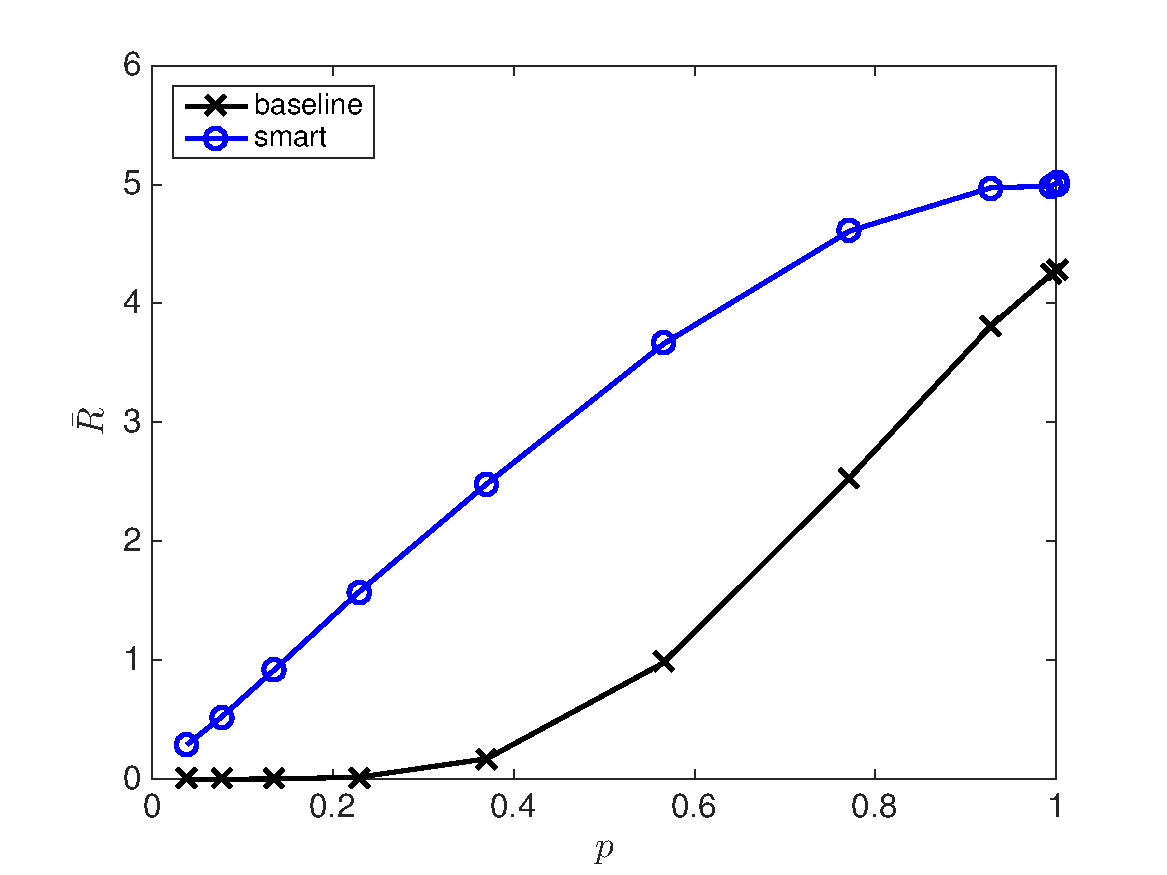
\includegraphics[scale=0.5]{R_p_sym.pdf}
\caption{Throughout v.s. Channel reliability}
\label{smart and baseline sym}
\end{figure}

\begin{figure}[htbp]
\centering
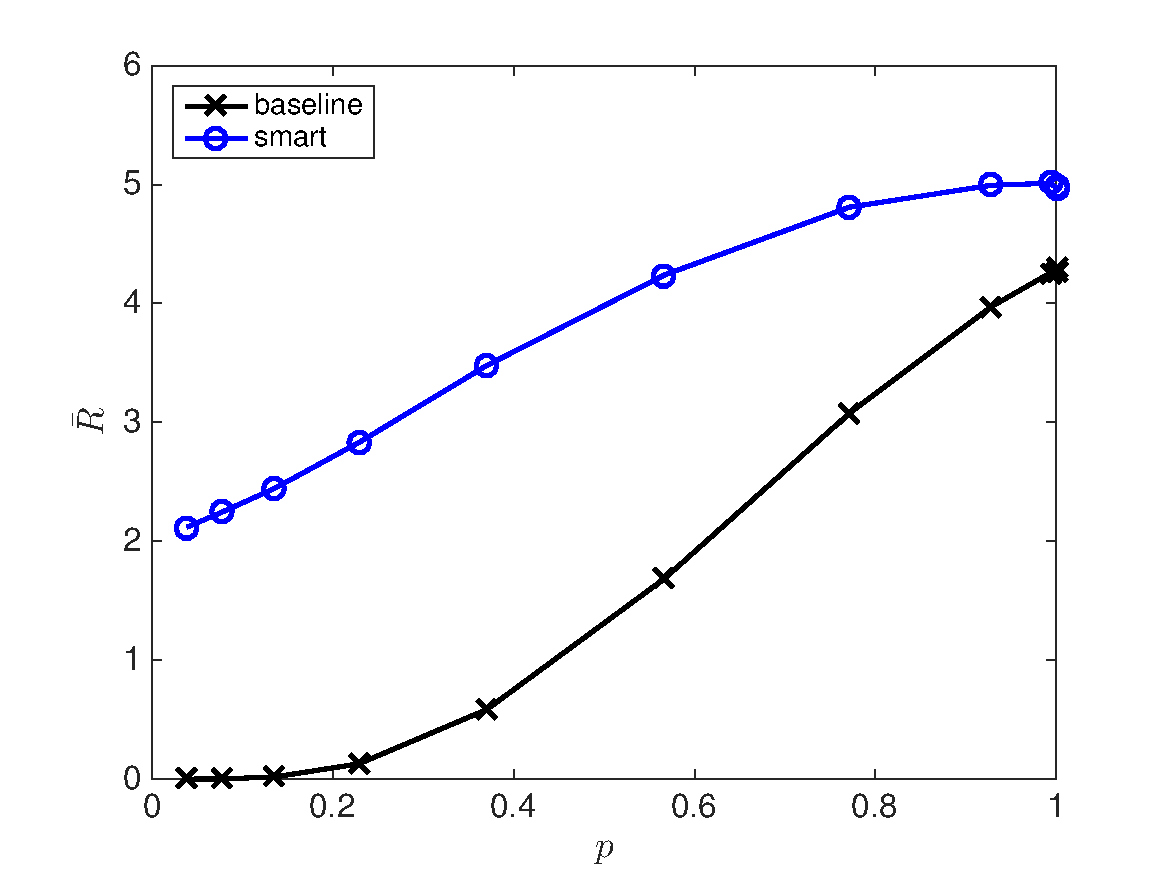
\includegraphics[scale=0.5]{R_p_asym.pdf}
\caption{Throughout v.s. Channel reliability}
\label{smart and baseline asym}
\end{figure}



\begin{comment}

\begin{figure}[htbp]
\centering
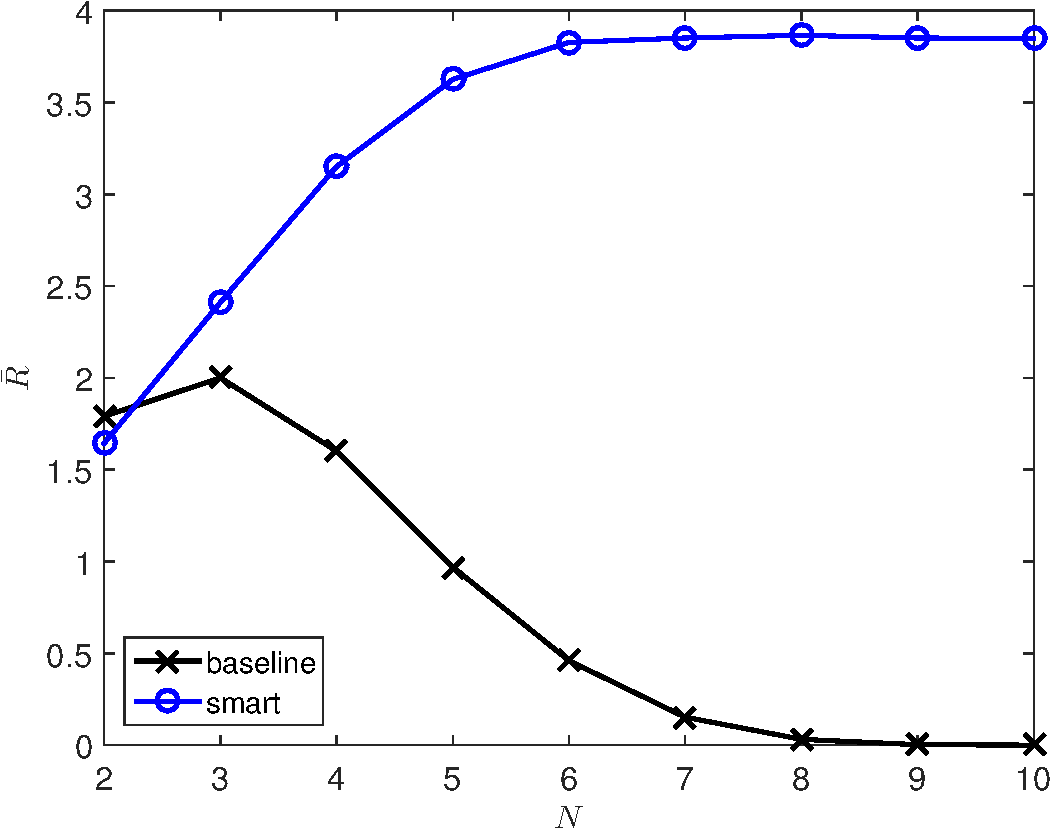
\includegraphics[scale=0.5]{R_N_sym.pdf}
\caption{Throughout v.s. Channel reliability}
\label{smart and baseline sym}
\end{figure}

\begin{figure}[htbp]
\centering
\includegraphics[scale=0.5]{R_N_asym.pdf}
\caption{Throughout v.s. Channel reliability}
\label{smart and baseline sym}
\end{figure}

\begin{figure}[htbp]
\centering
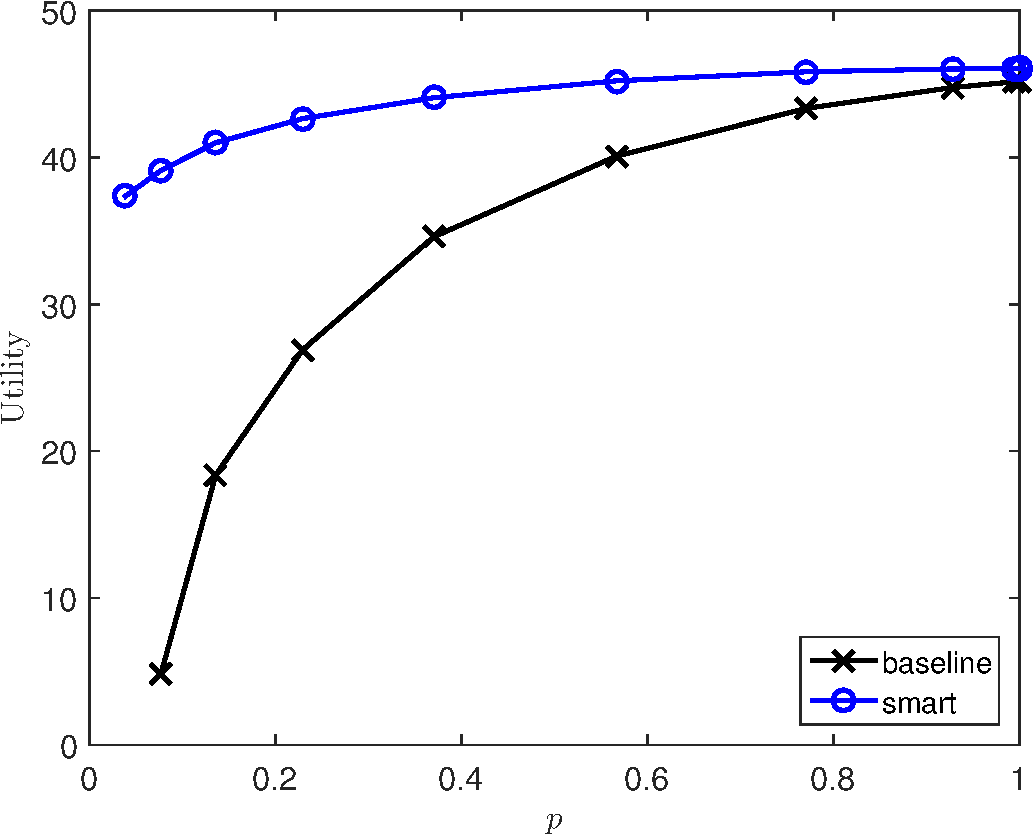
\includegraphics[scale=0.5]{U_p_asym.pdf}
\caption{Throughout v.s. Channel reliability}
\label{smart and baseline sym}
\end{figure}

\end{comment}



\begin{figure}[htbp]
\centering
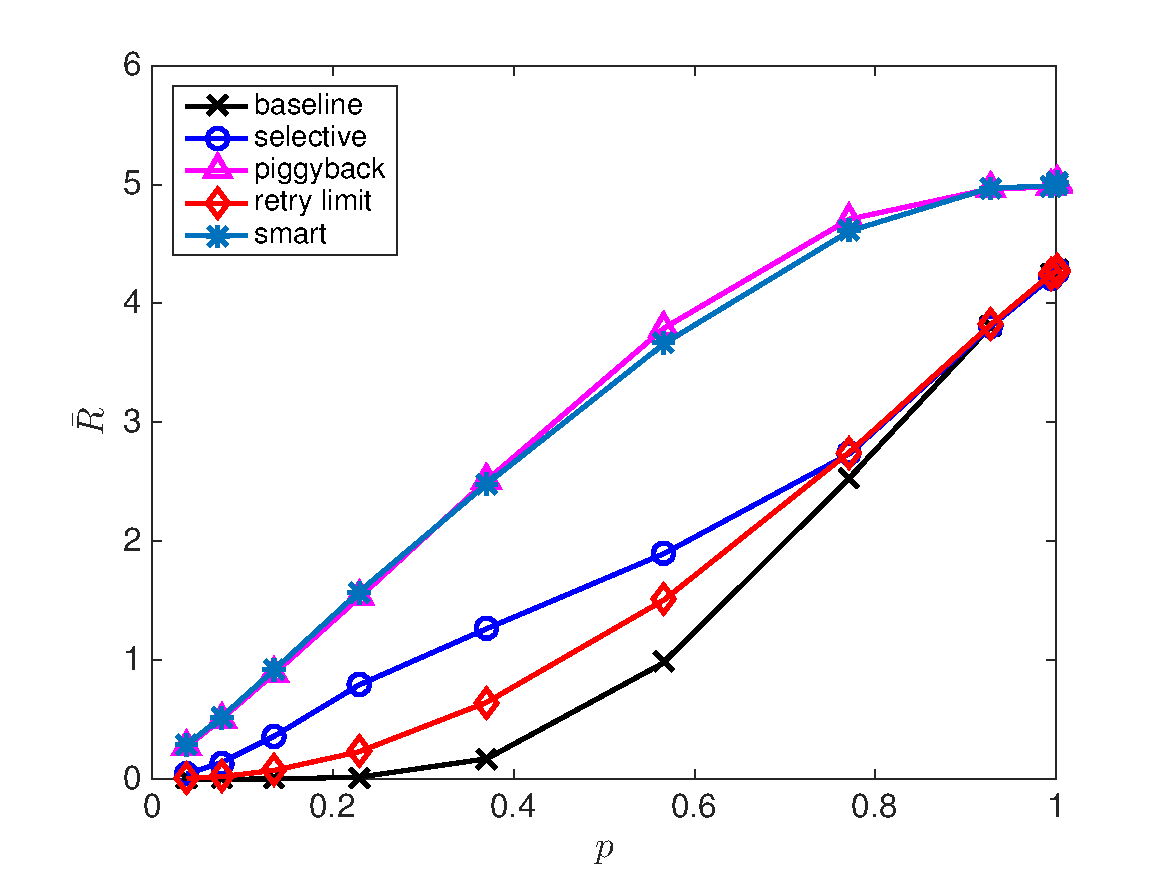
\includegraphics[scale=0.5]{3policycompare_sym.pdf}
\caption{Three Policies Under Symmetric Channel}
\label{Three Policies Under Symmetric Channel}
\end{figure}

\begin{figure}[htbp]
\centering
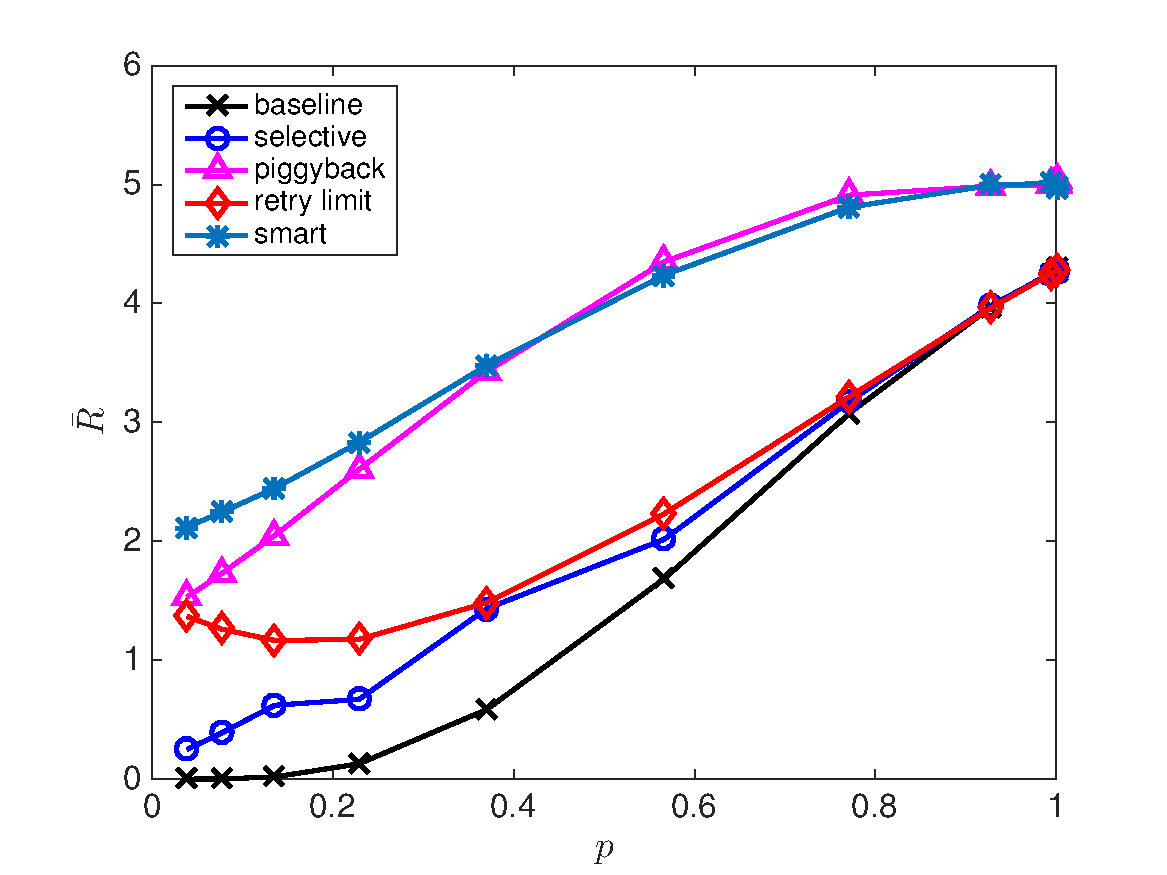
\includegraphics[scale=0.5]{3policycompare_asym.pdf}
\caption{Three Policies Under Asymmetric Channel}
\label{Three Policies Under Asymmetric Channel}
\end{figure}

\begin{figure}[htbp]
\centering
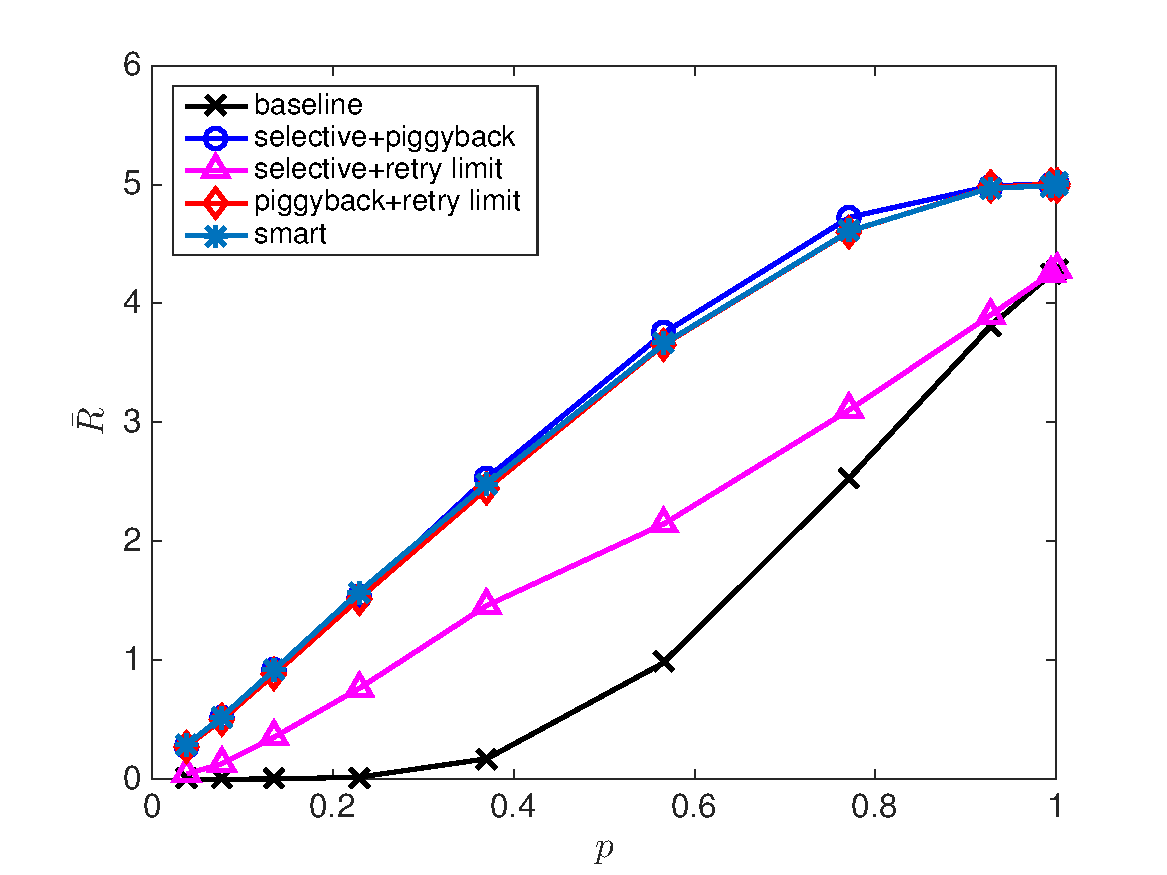
\includegraphics[scale=0.5]{sym_threecombinepolicys.pdf}
\caption{Combined Policies Under Symmetric Channel}
\label{Combined Policies Under Symmetric Channel}
\end{figure}

\begin{figure}[htbp]
\centering
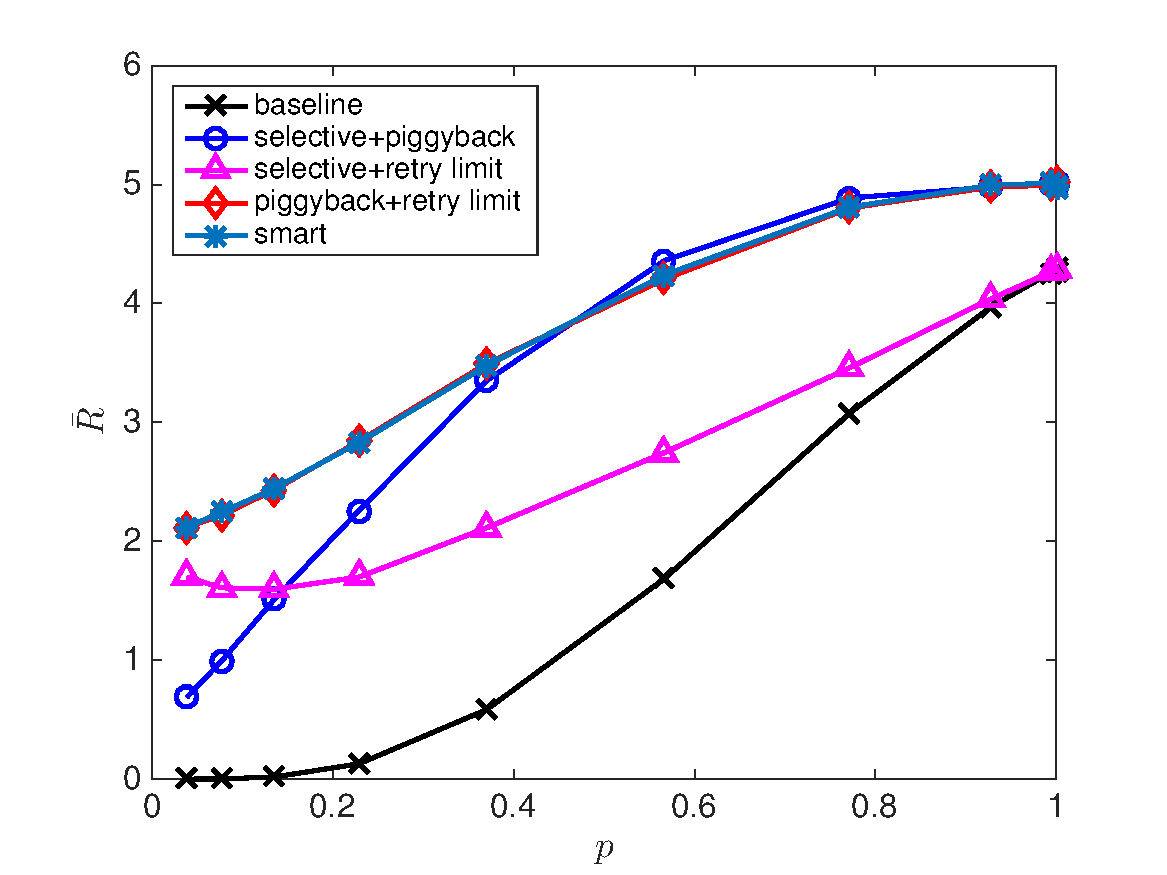
\includegraphics[scale=0.5]{asym_threecombinepolicys.pdf}
\caption{Combined Policies Under Asymmetric Channel}
\label{Combined Policies Under Asymmetric Channel}
\end{figure}


\section{Conclusion}
The baseline policy incurs huge overhead especially with large $N$ and poor channel. Our smart policy incorporates selective polling, piggybacking, and retry limit to improve the performance. Simulation shows our smart policy outperforms the baseline policy in terms of timely-throughput and network utility.


\end{document}